\documentclass[12pt]{standalone}
\usepackage{subcaption}
\usepackage{tikz}

\begin{document}
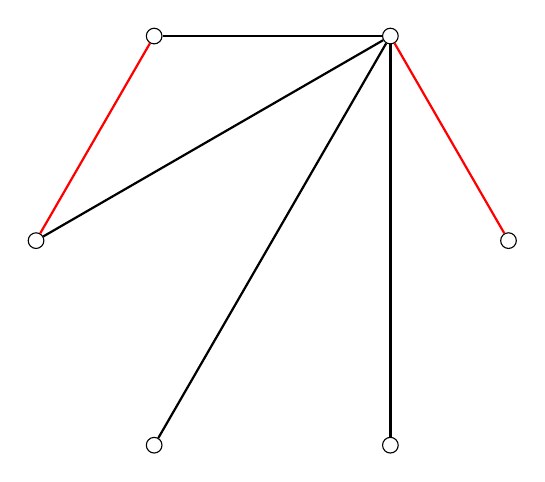
\begin{tikzpicture}[scale=1.5]
    \foreach \i in {1,2,3,4,5,6}
    \node[circle, draw, inner sep=2pt] (node\i) at (\i*60:2cm) {};

    \foreach \source/\dest/\edgecolor in {1/2/black,1/3/black,1/4/black,1/5/black,1/6/red,2/3/red}
    \draw[thick, \edgecolor] (node\source) -- (node\dest);
\end{tikzpicture}
\hspace{20pt}
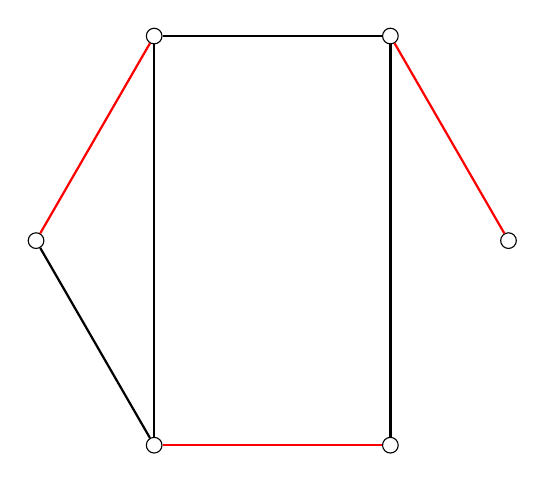
\begin{tikzpicture}[scale=1.5]
    \foreach \i in {1,2,3,4,5,6}
    \node[circle, draw, inner sep=2pt] (node\i) at (\i*60:2cm) {};

    \foreach \source/\dest/\edgecolor in {1/2/black,2/3/red,3/4/black,4/5/red,2/4/black,1/5/black,1/6/red}
    \draw[thick, \edgecolor] (node\source) -- (node\dest);
\end{tikzpicture}
\hspace{20pt}
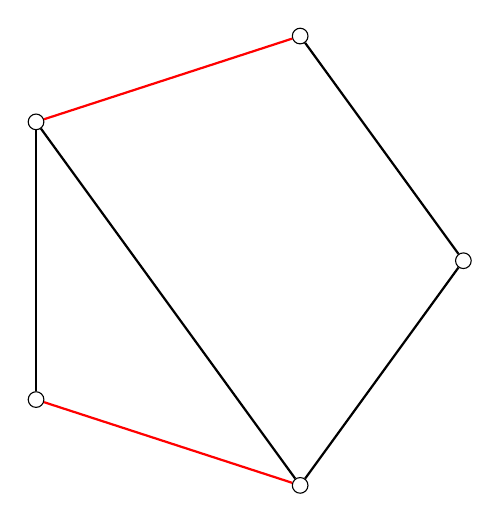
\begin{tikzpicture}[scale=1.5]
    \foreach \i in {1,2,3,4,5}
    \node[circle, draw, inner sep=2pt] (node\i) at (\i*72:2cm) {};

    \foreach \source/\dest/\edgecolor in {1/2/red,2/3/black,3/4/red,4/5/black,2/4/black,1/5/black}
    \draw[thick, \edgecolor] (node\source) -- (node\dest);
\end{tikzpicture}
\end{document}
